\chapter{Discussion of results} \label{cha:Discussion-of-results}

\section{Preliminary results} \label{sec:Preliminary-results}

Due to the low thrust of spacecraft \BW, it is expected that a substantial part of the orbit raising will be achieved by exploiting gravitational assists from the Moon. This technique has been well studied, although previous higher-thrust missions did not find it efficient to attempt more than one or two lunar resonances. \textcite{Kemble2006} explains that \enquote{It is possible to utilise lunar gravity to assist in the orbit raising prior to lunar encounter. This takes the form of a \emph{gravitational pumping} effect if the correct phase with respect to the Moon can be established}. He goes on to quantify that \enquote{A typical $\Delta V$ saving of 800~ms$^{-1}$ is obtained by use of lunar gravity assist}. Due to the extended duration of \BW's transit, more lunar resonances should be possible than in a \enquote{typical} scenario, so this should reduce the required delta-v for \BW's ascent from GTO to lunar orbit from 4.1~kms$^{-1}$ to less than 3.3~kms$^{-1}$.

Because lunar gravitational assists provide delta-v without fuel expenditure, they should be implicitly accounted for during optimisation. Preliminary results have already shown this to be the case, as seen in \autoref{fig:Lunar_resonance}. From an initial orbit of 180,000~km (semi-cis-lunar, representing the later stages of the transfer to highlight the lunar assist) the spacecraft takes two orbits to align its phase with the Moon, then receives a very apparent boost purely from the Moon's gravity.

\begin{figure}
\begin{center}
%\includegraphics[width=\textwidth,clip,trim=60 45 0 0]{Images/Low-thrust-Moon-transfer.jpg}
\end{center}
\caption{Preliminary orbit raising. Plot exported from ASTOS.}
\label{fig:Lunar_resonance}
\end{figure}

Regarding the thrust profile, it is well known that thrusting at particular points in the orbit are more efficient than others. \textcite{Kemble2006} once again explains, \enquote{Insertion of coast arcs allows the apogee raising input to be concentrated closer to perigee and hence increase the efficiency of the transfer (in terms of $\Delta V$ required)}. The reason for concentrating thrust near the perigee is known as the Oberth effect: over a period of thrusting, the specific orbital energy gained per unit delta-v exerted is equal to the instantaneous speed. Therefore thrusting is more efficient at high speed, which occurs at periapsis.
 
The resultant effect on the trajectory is that when variable thrust is implemented, the majority of the thrusting should occur near perigee; there should be an inverse relationship between thrust magnitude and orbital radius. The reverse seems apparent in \autoref{fig:Thrust_profile}, where smooth thrust input parabola appear to map points of greater orbital radius. This will be further investigated. It is likely that the observed variations in thrust magnitude are relatively insignificant (the magnitude is 6.31625$\pm$0.002~mN, so the variations represent only 0.03\%).

\begin{figure}
\begin{center}
%\includegraphics[width=\textwidth]{Images/thrust-vs-time.jpg}
\end{center}
\caption{Thrust exerted by \BW\ during the orbit raising. Plot exported from ASTOS.}
\label{fig:Thrust_profile}
\end{figure}

% Continuous thrust (tangential to the orbital radius) leads to circular trajectories because an eccentric starting trajectory spends more time at apoapsis than periapsis; hence more thrusting occurs at apoapsis than periapsis. As demonstrated by a Hohmann transfer, thrusting at apoapsis circularises the orbit.

This preliminary optimisation included no complex constraints on the thrusting profile such as cycling due to battery charging, Earth shadow or ground station communications. Implementing constraints such as these will require integration of the attitude control system to orient the spacecraft appropriately for battery charging or ground station communication, resulting in a much more complex pitch profile than that seen in \autoref{fig:BW1-Pitch}. The cycling observed in the figure is due to the elliptical orbit; at apogee and perigee the spacecraft is travelling perpendicularly to its position vector, resulting in a pitch angle of zero. As it travels towards the Earth, it has negative pitch angle, and positive pitch as it travels away again.
 
\begin{figure}
\begin{center}
%\includegraphics[width=\textwidth]{Images/pitch-vs-time.jpg}
\end{center}
\caption{Pitch angle of \BW\ during the orbit raising. Plot exported from ASTOS.}
\label{fig:BW1-Pitch}
\end{figure}

As observed in \autoref{fig:Thrust_profile} the thrust of \BW\ is almost constant throughout this simplified scenario. Consequently the traditional parameter for aircraft performance, thrust-to-weight ratio, seen in \autoref{fig:BW1-T/W-ratio}, is dominated by the changing effective weight, as the spacecraft moves closer to the Earth and then away again.

\begin{figure}
\begin{center}
%\includegraphics[width=\textwidth]{Images/thrust-to-weight-and-radius-vs-time.jpg}
\end{center}
\caption{\BW\ T/W ratio compared to radial position during the orbit raising. Plot exported from ASTOS.}
\label{fig:BW1-T/W-ratio}
\end{figure}

\section{Anticipated results} \label{sec:Anticipated-results}

A spacecraft orbiting the Moon (in the same direction as the Moon orbits the Earth) undergoes a period of low velocity relative to the Earth every time it is on the Earthward side of the Moon. A spacecraft orbiting the Earth in a highly elliptical orbit undergoes a period of low velocity relative to the Earth when it reaches apoapsis, which is conveniently also the furthest point from the Earth, as shown in \autoref{fig:Apoapsis-and-periapsis}. Therefore the trajectory is expected to deliver the spacecraft at apoapsis to a \enquote{stationary point} in the intended lunar orbit, such that the Moon's gravity will then pull it into a steady lunar orbit, avoiding the need for a high-thrust capture maneuvre.

\begin{figure}
\begin{center}
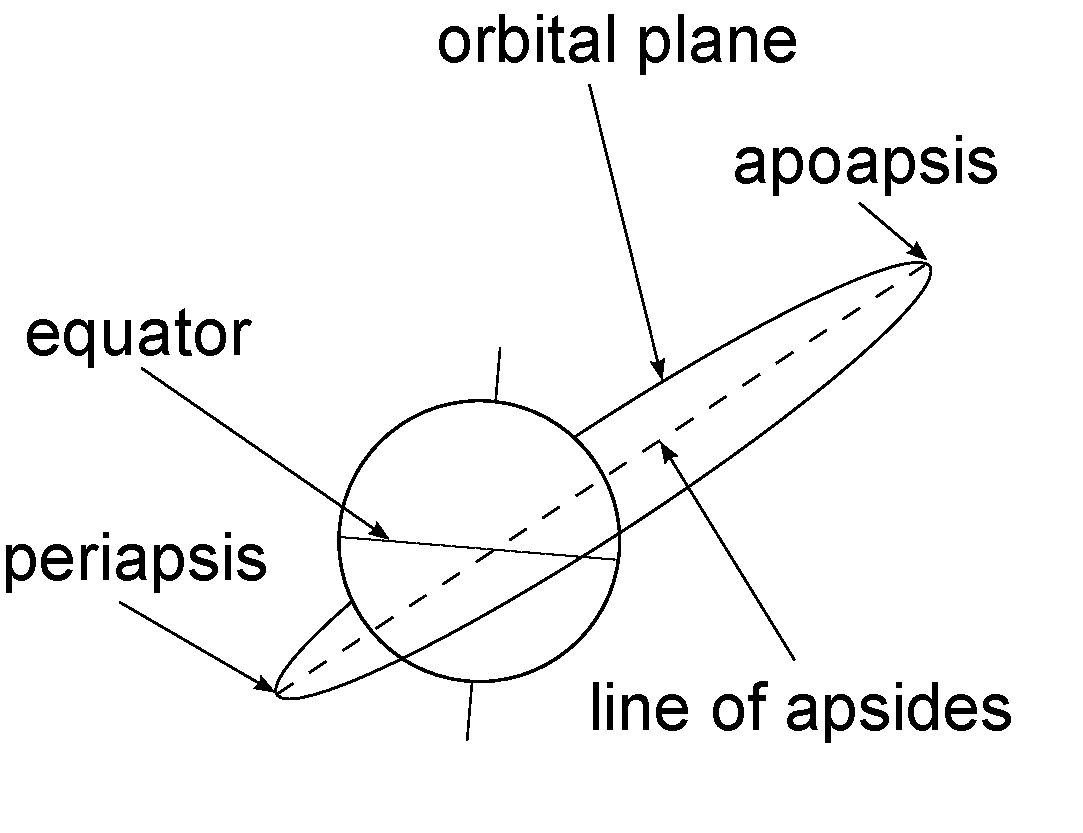
\includegraphics[scale=0.4]{Images/apsides.pdf}
\end{center}
\caption{Apoapsis and periapsis.}
\label{fig:Apoapsis-and-periapsis}
\end{figure}

To maximise the gravitational effect of the Moon on the spacecraft, it should be phase-locked with respect to the Moon's orbit. However, this would require constantly adjusting the orbital line of apsides, which is a high delta-v maneuvre. Gravitational resonance is generally exploited by pointing the apoapsis towards the Moon's ascending node (to remove any dependence on inclination) and adjust the orbital period to resonate with the Moon (that is, the spacecraft completes two orbits to every lunar orbit, or three orbits to every lunar orbit, or five orbits to every two lunar orbits, etcetera). However, based on the unique thrusting constraints of \BW, an alternative optimal scenario may be to maintain the fastest part of the orbit (periapsis) within the Earth's shadow (eclipse), to minimise the amount of time that the craft cannot charge its batteries. In this scenario the spacecraft should also thrust as it passes through the eclipse since it cannot recharge during this time, and thrusting will help it to escape the eclipse as quickly as possible. It will also be interesting to see whether it is optimal to correct inclination, apoapsis or eccentricity first, or whether the optimal solution adjusts all of these parameters simultaneously.
 
% It is well known how to most efficiently control various aspects of an orbit by thrusting at fortuitous times: increasing apoapsis efficiently by thrusting near periapsis, inclination by thrusting out of the orbital plane at apoapsis, and so forth, as anticipated by \textcite{Dachwald2007} in their discussion of optimisation results. \citet{Gao2008} outlines a convenient mathematical model to generate continuous, smooth parameters describing thrust steering, which can easily be used in an optimisation engine.
 
% quantify stochastic & deterministic inputs, robustness

\section{Ascent} Initial guess, simulation, optimisation
how initial guess was developed, simulation run from starting conditions of mission architecture with initial guess for thrust profile until approaching termination condition to get initial guess for delta L. Graph of perturbations on optimised trajectory, thrust profile of optimised trajectory, not significant - therefore just adjusting launch date. Only affects position of moon?
compare fuel used with initial guess.
then - ascent with variable thrust
then - ascent with power constraint
oscillations between ur and utheta - similar result to that discovered by \textcite{Betts2003}
\textcite{Edelbaum1964} gives an outline of some optimal low-thrust maneouvres (a, e, plane changes)
arg of periapsis most efficiently changed at low eccentricity, inclination at high eccentricity, RAAN constant, a at periapsis.

\section{Cruise}
Initial guess, simulation, optimisation
Thrust profile - demonstrating Oberth affect by thrusting more at periapsis.
Multiple different initial guesses based on power - leading to lunar capture
optimising cruise phase forwards to given termination condition (SOI) causes numerical errors (gets pulled into lunar orbit and so L (ECI) is no longer independent, or gets thrown into escape trajectory and so L (ECI) no longer increases, or ...).
tried backward propagating from final orbit, but thrusting tangentially does not change inclination so it is difficult to achieve the nearly polar orbit required.
found that, due to the similar launch inclination coupled with the slow ascent leading to many lunar assists, almost any launch will end up near the Moon. The problem thus becomes ensuring lunar capture, rather than a lunar slingshot into an Earth-escape trajectory. This was achieved by modelling the scenario in STK, assigning arbitrary values for $\omega$ and $\Omega$, and then using STK's BVP solver to establish a feasible initial guess for the optimiser. 
Also, very difficult to achieve polar lunar orbit with forwards propagation. Backwards propagation from lunar orbit will ascend in polar orbit, until lunar escape velocity achieved. Provided it escapes in the right direction (and doesn't achieve Earth escape velocity) it goes into high Earth orbit near lunar inclination - which is relatively near to launch inclination. Try backwards propagation for the whole transfer?
circular orbit - rendezvous with moon can't really be scheduled, it will happen inevitably. can schedule effect of rendezvous perhaps? change inclination/eccentricity etc?

\section{Capture}
Initial guess, simulation, optimisation
Increase phase duration until it gets close to escape.
Adjust starting date until point where difference between satellite phase and lunar phase changes direction (i.e. satellite is near the same orbit as the moon) is close to 0\degrees.

\section{Descent}
Initial guess, simulation, optimisation

\section{Science}
Initial guess, simulation
plot of science orbit in LCI
plot of science orbit in SEL!!!! 

\section{Validation}
For obvious reasons there have been few experimental flights to validate low-thrust trajectory theory, and no flight testing is possible to verify this particular proposed trajectory. However, the laws governing forces acting on spacecraft are known better than other theory, for example atmospheric trajectories. This trajectory was imported into STK (Satellite Tool Kit), the most widely used industry tool for modelling spacecraft trajectories, provided by AGI (Analytical Graphics, Inc.). There were minor differences as seen in \ref{fig:STK-verification} due to different orders of complexity in Earth oblateness and the algorithms used to calculate third body perturbations, but these differences were essentially negligible as seen in \ref{fig:STK-error}.

Compare the objective function score against a few other cases.
Of course, the ultimate validation is the launch. Unfortunately at this stage in the design, there is still no fixed launch date scheduled.
Final optimal solution.
Why it is optimal – comparison of objective function (fuel) against other profiles (eg. Pure thrust)
Comment on gravitational assists, thrust profile (Oberth affect – thrusting more at periapsis).
Requires addition of thrust magnitude as a parameter. Minimal work.
Link in to battery level?! Much work.
Verification – STK, matlab?
\textcite{Pollard2000} describes a numer of steering programs for low thrust orbital maneuvres.
Optimisation run from 15/4/2011 to 21/4/2011. neglected to constrain mass starting value for ascent phase. optimiser found best way to maximise final mass was to increase the initial mass as far as possible (hard limit set by parameter bounds for affine transform). suggests a continuous optimisation to higher mass. computation took so long perhaps because the entire trajectory changed every time the mass changed? just VAB escape so minor changes probably less significant than later on (closer to moon). Less stiff problem.
explanation of optimal thrust strategies - \textcite{Herbiniere2000}
verify by putting thrust profile in STK (and get nice videos!)
compare fuel used to SMART-1 (BW1 average Isp is lowered by use of arcjet)
compare fuel used to initial guess
get cruise phase to terminate at apoapsis for capture
ascent phase not so important, since it keeps going in circles around the same focus anyway.
cruise phase adjusts launch date for lunar resonances (thrust profile not as important)
ascent phase just changes thrust profile, launch date not as important since it doesn't get near Moon (therefore individual phase optimisation launch date not important; combined scenario launch date should be dominated by cruise phase)
compare fuel use to SMART-1 (lower Isp because of arcjet)
compare fuel use to initial guess

